\documentclass{scrreprt}
\usepackage{listings}
\usepackage{underscore}
\usepackage[T2A]{fontenc}
\usepackage[utf8]{inputenc}
\usepackage[russian]{babel}
\date{}
\usepackage{geometry}
\usepackage{graphicx}
\usepackage{array}
\usepackage{tabularx}	
\usepackage{enumitem}
\usepackage{graphicx}
\usepackage{subcaption}


\geometry{
	a4paper,
	left=30mm,
	right=15mm,
	top=20mm,
	bottom=20mm
}

\usepackage{hyperref}
\begin{document}
\begin{center}
	\textbf{Министерство науки и высшего образования Российской Федерации} \\
	\textbf{Федеральное государственное автономное образовательное учреждение высшего} \\
	\textbf{образования} \\
	«Национальный исследовательский университет ИТМО» \\
	
	\vspace{1cm}
	
	\textbf{Факультет Программной инженерии и компьютерной техники} \\
	
	\vspace{2cm}
	
	\textbf{Лабораторная работа №1} \\
	
	\vspace{1cm}
	
	по дисциплине «Основы программной инженерии» \\
	
	\vspace{1cm}
	
	Вариант: 911 \\
	
	\vspace{2cm}
	
\begin{flushright}
	\textbf{Преподаватель:} \\
	Карташев Владимир Сергеевич \\
	
	\vspace{0.5cm}
	
	\textbf{Выполнил:} \\
	Ребрый Егор Сергеевич \\
	
	\vspace{0.5cm}
	
	\textbf{Группа:} \\
	Р3209 \\
\end{flushright}
	
	\vfill
	
	Санкт-Петербург, 2025 \\
\end{center}

\tableofcontents

\chapter{Introduction}

\section{Purpose}
Целью данного документа является предоставление подробного описания требований к программному обеспечению «РБК Недвижимость». Он проиллюстрирует цель, объяснит системные ограничения, интерфейс и взаимодействие с другими
внешними приложениями. Этот документ в первую очередь предназначен для предложения заказчику и в качестве справочного материала для команды разработчиков.

\section{Project Scope}
Документ относится к разрабатываемому веб-сайту https://realty.rbc.ru/ - аналитическому и новостному порталу о недвижимости, объединяющий актуальные новости, рыночные данные. Описанная в этом документе система позволит пользователям использовать сайт для просмотра и публикации статей и новостей о недвижимости.

\section{Definitions, Acronyms and Abbreviations}
\begin{enumerate}
\item\textbf{DESC} – \textbf{Desc}ription (Описание).

\item\textbf{RAT} – \textbf{Rat}ional (Рациональное, отвечает на вопрос 'Зачем нужно то или иное требование').

\item\textbf{DEP} – \textbf{Dep}endencies (Зависимости).

\item\textbf{UX} – \textbf{U}ser E\textbf{x}perience (пользовательский опыт, удобство взаимодействия с интерфейсом).

\item\textbf{РБК} – \textbf{Р}ос\textbf{б}изнес\textbf{к}онсалтинг (российское медиа и информационное агентство).

\item\textbf{CMS} – \textbf{C}ontent \textbf{M}anagement \textbf{S}ystem (система управления контентом, нужна для простого добавления контента на сайт редакторами).

\item\textbf{SEO} – \textbf{S}earch \textbf{E}ngine \textbf{O}ptimization (оптимизация сайта для поисковых систем).

\item\textbf{Мультимедиа} – контент, сочетающий текст, графику, звук и вид\textbf{}ео.

\item\textbf{Javascript} – язык программирования для создания интерактивных веб-страниц.

\item\textbf{Cookies} – небольшие текстовые файлы, хранящие данные о пользователе на его устройстве.

\item\textbf{HTML} – \textbf{H}yper\textbf{T}ext \textbf{M}arkup \textbf{L}anguage (язык разметки веб-страниц).

\item\textbf{CSS} – \textbf{C}ascading \textbf{S}tyle \textbf{S}heets (язык стилей для оформления HTML-документов).

\item\textbf{Интернет} – глобальная сеть взаимосвязанных компьютеров и серверов.

\item\textbf{МБ (MB)} – \textbf{М}ега\textbf{б}айт (единица измерения данных, 1 МБ = 1024 КБ).

\item\textbf{ТБ (TB)} – \textbf{Т}ера\textbf{б}айт (1 ТБ = 1024 ГБ).

\item\textbf{Статья/пост} – публикация в блоге, СМИ или соцсети.

\item\textbf{ВКонтакте (ВК/VK)} – российская социальная сеть.

\item\textbf{VK ID} – универсальный аккаунт для авторизации в сервисах VK.

\item\textbf{Одноклассники} – российская социальная сеть.

\item\textbf{Telegram} – мессенджер.

\item\textbf{Email} – \textbf{E}lectronic \textbf{mail} (электронная почта).

\item\textbf{Пароль} – секретная комбинация символов для доступа к аккаунту.

\item\textbf{Аккаунт} – учётная запись пользователя в системе.

\item\textbf{OAuth} – протокол авторизации через сторонние сервисы (например, вход через Google, VK ID).

\item\textbf{FR} – \textbf{F}unctional \textbf{R}equirement (функциональное требование).

\item\textbf{QR} – \textbf{Q}uality \textbf{R}equirement (требование качества).

\item\textbf{РБК ТВ} – телевизионный канал медиахолдинга РБК.

\item\textbf{Инфографика} – графическое представление информации.

\item\textbf{Подписка} – оформление регулярного доступа к контенту или услугам.

\item\textbf{WYSIWYG} – \textbf{W}hat \textbf{Y}ou \textbf{S}ee \textbf{I}s \textbf{W}hat \textbf{Y}ou \textbf{G}et (визуальный редактор, где текст отображается так же, как и в публикации).

\item\textbf{Тег} – метка у контента.

\item\textbf{HTML-тег} – элемент разметки в HTML.

\item\textbf{Мета-тег} – HTML-тег с метаданными о странице (например, <meta name="description">).

\item\textbf{Alt-текст} – альтернативный текст для изображений.

\item\textbf{Модерация} – проверка контента на соответствие правилам платформы.

\item\textbf{База данных (БД)} – структурированное хранилище информации (например, MySQL, PostgreSQL).

\item\textbf{DDoS-атака} – \textbf{D}istributed \textbf{D}enial \textbf{o}f \textbf{S}ervice (атака на сервер для его перегрузки).

\item\textbf{CSV} – \textbf{C}omma-\textbf{S}eparated \textbf{V}alues (текстовый формат табличных данных).

\item\textbf{Гайдлайн} – руководство по стилю или правилам оформления.

\item\textbf{Шрифт} – графический набор символов определённого стиля.

\item\textbf{Бренд} – уникальный образ компании или продукта.

\item\textbf{MTTR} – \textbf{M}ean \textbf{T}ime \textbf{T}o \textbf{R}epair (среднее время восстановления после сбоя).

\item\textbf{CDN} – \textbf{C}ontent \textbf{D}elivery \textbf{N}etwork (сеть доставки контента для ускорения загрузки).

\item\textbf{API} – \textbf{A}pplication \textbf{P}rogramming \textbf{I}nterface (интерфейс для взаимодействия программ).

\item\textbf{RPS} – \textbf{R}equests \textbf{P}er \textbf{S}econd (количество запросов в секунду).

\item\textbf{HTTP} – \textbf{H}yper\textbf{T}ext \textbf{T}ransfer \textbf{P}rotocol (протокол передачи данных).

\item\textbf{HTTPS} – \textbf{HTTP} \textbf{S}ecure (защищённая версия HTTP с шифрованием).

\item\textbf{iOS} – операционная система Apple.

\item\textbf{Android} – мобильная операционная система от Google.

\item\textbf{ES} – \textbf{E}cma\textbf{S}cript (стандарт JavaScript).

\item\textbf{Swiper.js} – JavaScript-библиотека для создания слайдеров.

\item\textbf{RESTful} – архитектурный стиль API, основанный на HTTP-методах и JSON.

\item\textbf{GET/POST/PUT/DELETE} – HTTP-методы для запросов (получение, отправка, обновление, удаление данных).

\item\textbf{JSON} – \textbf{J}ava\textbf{S}cript \textbf{O}bject \textbf{N}otation (текстовый формат обмена данными).

\item\textbf{XML} – e\textbf{X}tensible \textbf{M}arkup \textbf{L}anguage (язык разметки для структурированных данных).

\item\textbf{jQuery} – популярная JavaScript-библиотека для упрощения работы.
\end{enumerate}
\section{Intended Audience and Reading Suggestions}
Данный документ предназначен для:
\begin{itemize}
	\item Руководителя проекта
	\item Разработчиков
	\item Тестировщиков
	\item Сотрудников отдела маркетинга
	\item Дизайнеров и UX-аналитиков
\end{itemize}

\section{References}
\begin{enumerate}
	\item IEEE Software Engineering Standards Committee, “IEEE Std 830-1998, IEEE Recommended
	Practice for Software Requirements Specifications”, October 20, 1998.
	\item Клименков С.В., Цопа Е.А.,Козин И.О. 'Конспект лекций по ОПИ v1.4', unpublished
	\item Robert Feldt
	'SRS Example'
	
	 https://www.cse.chalmers.se/~feldt/courses/reqeng/examples/srs_example_2010_group2.pdf
\end{enumerate}

\section{Overview}
Следующий раздел, Overall Description, представит общее описание разрабатываемого
продукта. В частности, опишет предполагаемый функционал продукта, различные
ограничения и зависимости на высоком уровне.
Третий раздел, Specific Requirements, содержит конкретное описание различных функций,
требований к удобству, безопасности и надежности, необходимых при разработке системы.
Также в нем указаны технологии, системы разработки и прочие инструменты,
предназначенные непосредственно для разработчиков.

\chapter{Overall Description}
В этом разделе будет дан обзор всей системы. Система будет объяснена в ее контексте, чтобы показать, как система взаимодействует с другими системами, и представить ее базовую функциональность. Также будет
описан тип заинтересованных лиц, которые будут использовать систему, и какая функциональность доступна для каждого типа. Наконец, будут представлены ограничения и предположения для 	системы.
\section{Product functions}

Разрабатываемая система должна предоставлять пользователям возможность
просматривать новости и статьи, делиться ими в
социальных сетях и на других площадкахи. Для
зарегистрированных пользователей должны быть доступно подключение рассылки и оформление подписок 'РБК Comfort', 'РБК Pro'.

\section{User characteristics}
Выделяются три основные категории пользователей, которые взаимодействуют с системой: обычные пользователи сайта, создатели статей и администраторы. Каждая группа пользователей обладает уникальными характеристиками и требованиями

\begin{enumerate}
\item Пользователи сайта (Гости и Авторизованные пользователи)

Эта группа ищет актуальные объявления, аналитику и новости. Они ожидают быстрой загрузки страниц и адаптивного дизайна под любые устройства. Гости могут свободно просматривать материалы, а зарегистрированные пользователи — подписываться на рассылку и оформлять подписки для получения аналитики от профессиональных инвесторов РБК. Ключевые требования — достоверность данных, интуитивная навигация и минимальное количество рекламы.

\item Создатели статей (Авторы, Редакторы)

Эта группа отвечает за наполнение сайта статьями, новостями и аналитическими обзорами. Они работают в CMS, добавляют текст, мультимедиа (фото, видео, инфографику) и настраивают SEO-параметры для продвижения. Им необходимы редактор с поддержкой форматирования, инструменты для совместной работы (например, черновики и согласование правок), а также возможность быстрой публикации. Также важна 	 защита от случайного нарушения авторских прав.

\item Администраторы (Системные администраторы, Технические специалисты)

Эта группа обеспечивают стабильную работу сайта: настраивают серверы, контролируют нагрузку, устраняют сбои и обновляют систему. Они управляют правами доступа (например, разграничивают роли авторов и редакторов), настраивают резервное копирование и защищают ресурс от атак. Для них критичны инструменты мониторинга (логи, метрики производительности), автоматизация рутинных задач (деплой, тестирование) и оперативное оповещение о критических инцидентах. Безопасность данных пользователей и отказоустойчивость инфраструктуры — ключевые приоритеты.

\end{enumerate}

\section{Constraints}

Браузер является ограничением для продукта. Поскольку для корректной работы сайта необходим JavaScript и Cookies, то браузер, используемый пользователем должен поддерживать Javascript и Cookies.

Интернет-соединение такжя является ограничением для продукта. Поскольку сайт извлекает данные из базы данных через Интернет, крайне важно, чтобы Интернет-соединение было стабильно и скорость была достаточна (рекомендуемая скорость: более 5 Мбит/с).

Кроме того, продукт ограничен емкостью базы данных. Поскольку сайт будет использоваться многими людьми, может потребоваться ставить в очередь входящие запросы и, следовательно, увеличивать время, необходимое для извлечения данных.

\section{Assumptions and Dependencies}

Главное предположение о продукте заключается в том, что он всегда будет использоваться на устройствах, которые имеют достаточную
производительность. Если у устройства недостаточно аппаратных ресурсов, доступных для сайта, например, пользователи могли выделить их другим приложениям или сайтам, могут быть сценарии, когда приложение
не работает так, как задумано, или даже не работает вообще.

\chapter{System Features}
В этом разделе содержатся все функциональные и качественные требования к системе. Он дает подробное описание системы и всех ее функций.
\section{User interfaces}
 В этом разделе дается подробное описание прототипа пользовательского интерфейса.
 
 Когда пользователь заходит на сайт он должен увидеть главную страницу(см Рис. 1), на которой должны отображаться:
 \begin{itemize}
 	\item Новые статьи
 	\item ТВ Эфир канала 'РБК ТВ'
 	\item Инфографика цен на квартиры в московских новостройках
 	\item Блок, в котором можно сортировать статьи по тегам
 	\item Кнопка для авторизации пользователя
 	\item Кнопка для поиска статей на сайте
 	\item Курс валют
 \end{itemize}
 
 Пользователь может открыть статью нажатием на неё. В статье (см Рис. 2) можно узнать:
 \begin{itemize}
 	\item Тег статьи
 	\item Время публикации
 	\item Количество просмотров
 	\item Автора статьи
 	\item Непосредственно текст и картинки в статье
 \end{itemize}
 
 Кроме того статьёй можно поделиться в социальных сетях, нажав на кнопку "Поделиться". В выпадающем списке(см Рис. 3) можно увидеть социальные сети, в которые можно поделиться статьёй.
 
 \begin{figure}
 	\centering
 	 \begin{subfigure}[b]{0.5\textwidth}
 		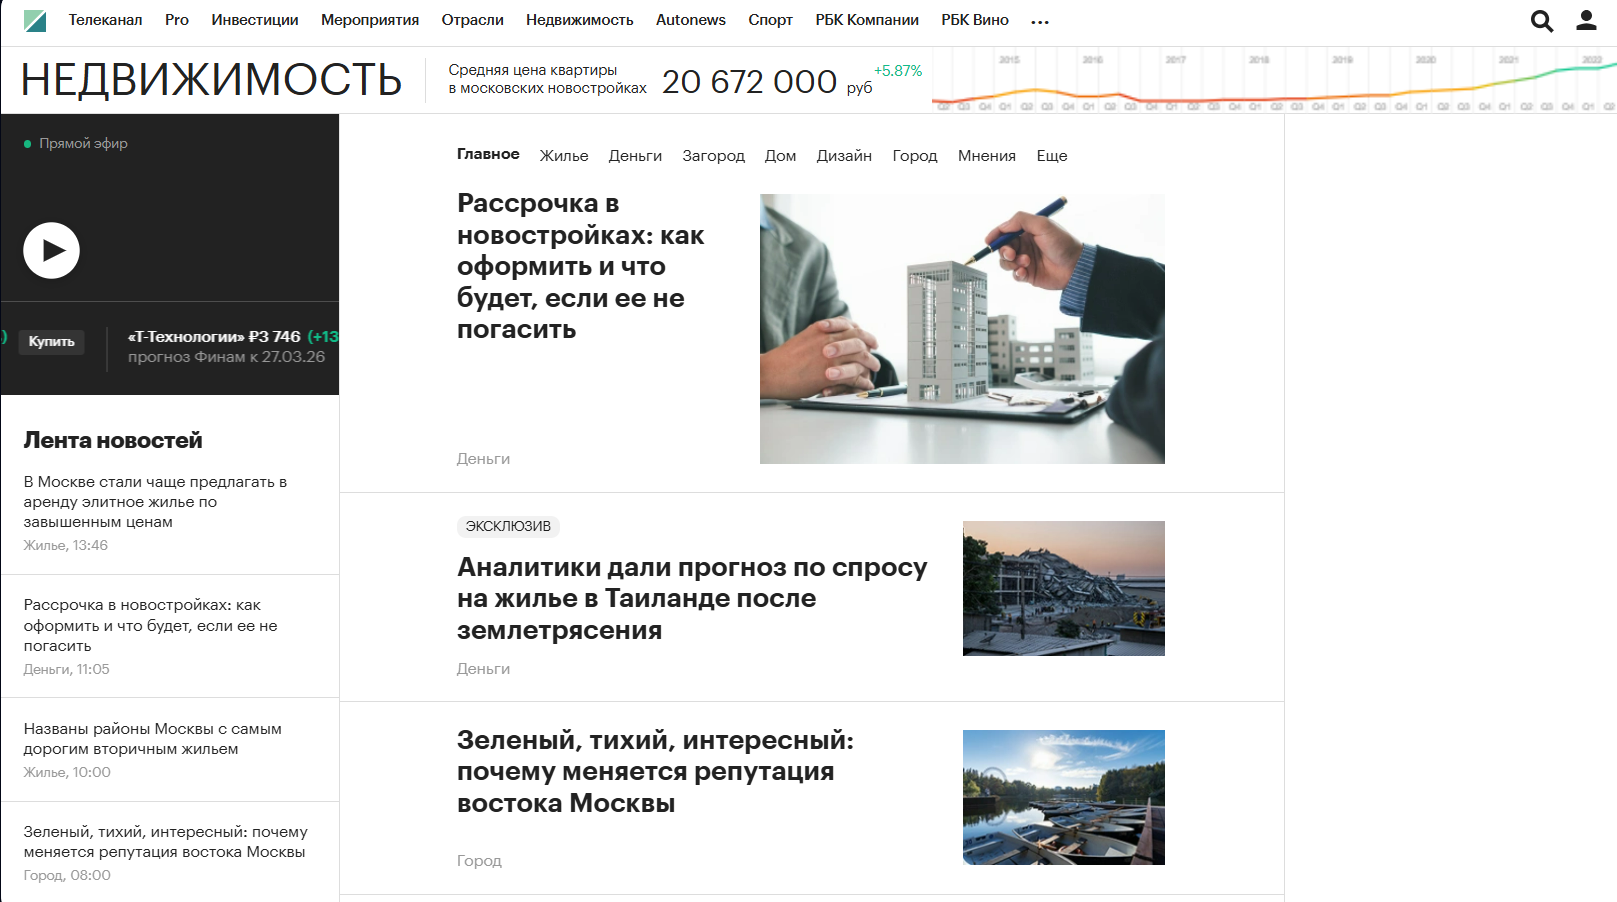
\includegraphics[width=\textwidth]{a}
 		\caption{Рис. 1} 
 	\end{subfigure}
 \end{figure}
 
 \begin{figure}[ht]
 	\centering
 	\hfill
 	\begin{subfigure}[b]{0.4\textwidth}
 		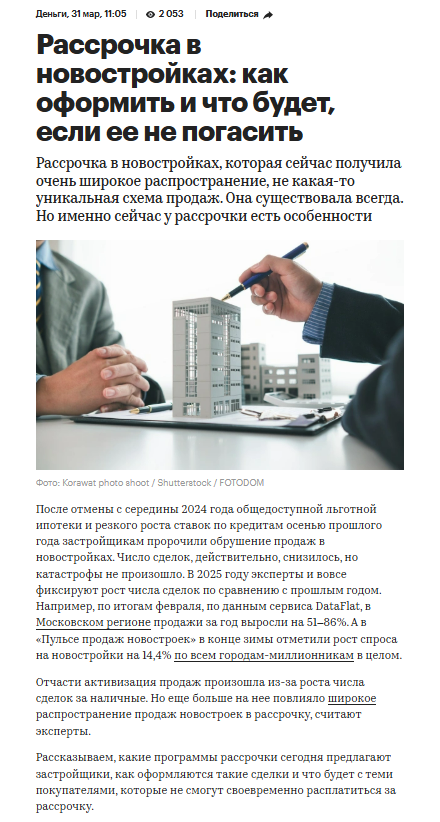
\includegraphics[width=\textwidth]{b}
 		\caption{Рис. 2}
 	\end{subfigure}
 	\hfill
 	\begin{subfigure}[b]{0.4\textwidth}
 		
\includegraphics[width=\textwidth]{c}
 		\caption{Рис. 3}
 	\end{subfigure}
 \end{figure}
 
 На главной странице можно нажать на кнопку авторизации и 'Вход'/'Регистрация', выбрав соответствующую опцию. На странице регистрации (см Рис. 4) можно зарегистрироваться с помощью email/пароль или VK ID, на странице входа (см Рис. 5) также можно войти с помощью email/пароль или VK ID.
 
 Авторизованный пользователь может войти в личный кабинет (см Рис. 6), где может поменять пароль, email и управлять картами.
  \begin{figure}[ht]
 	\centering
 	 \begin{subfigure}[b]{0.3\textwidth}
 		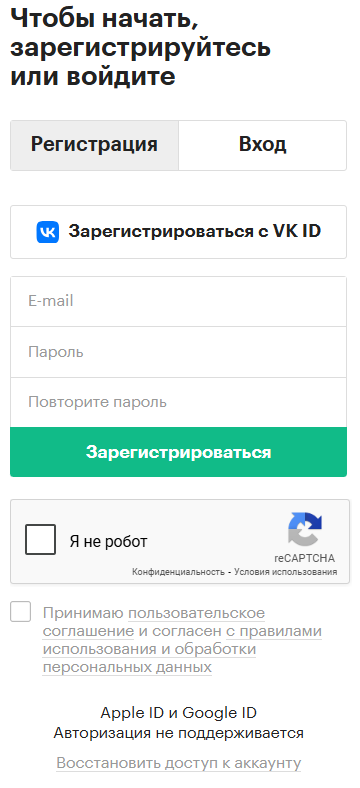
\includegraphics[width=\textwidth]{d}
 		\caption{Рис. 4} 
 	\end{subfigure}
 	\hfill
 	\begin{subfigure}[b]{0.3\textwidth}
 		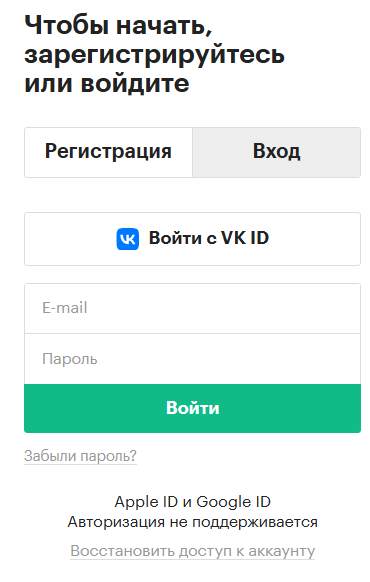
\includegraphics[width=\textwidth]{e}
 		\caption{Рис. 5}
 	\end{subfigure}
 	\hfill
 	\begin{subfigure}[b]{0.3\textwidth}
 		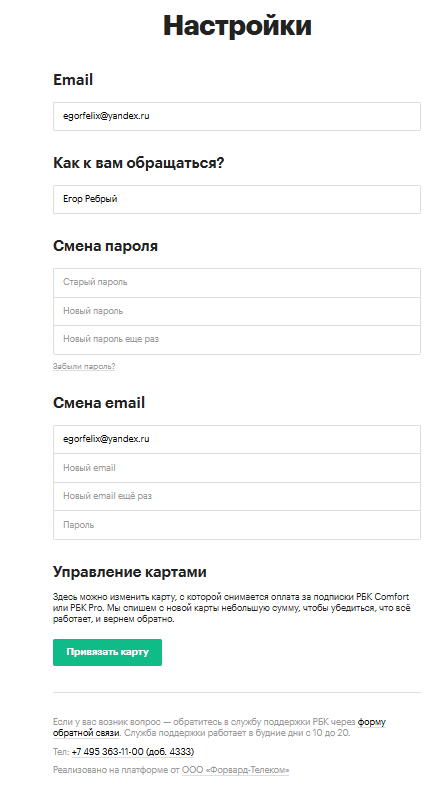
\includegraphics[width=\textwidth]{f}
 		\caption{Рис. 6}
 	\end{subfigure}
 \end{figure}
 \newpage
\section{Functional Requirements}
В этот раздел включены требования, определяющие все основные действия программной системы.
\subsection{Пользователи сайта}
\subsubsection{Functional requirement 1.1}
\textbf{ID: FR1}

TITLE: Просмотр статей о недвижимости

DESC: Система должна предоставлять функционал для того, чтобы пользователь мог просматривать опубликованные статьи, тесты, новости и аналитические материалы по тематике недвижимости. Максимум статей, доступных для просмотра на сайте - 30 штук. 

RAT: Основная функция сайта — предоставление информации о рынке 
недвижимости.

DEP: Нет
\subsubsection{Functional requirement 1.2}
\textbf{ID: FR2}

TITLE: Навигация по тегам

DESC: Система должна предоставлять функционал(на главной странице должен быть блок с возможностью выбора тега) для того, чтобы пользователь мог фильтровать статьи по тегам (например, 'Жилье', 'Деньги', 'Загород'). 

RAT: Упрощает поиск релевантного контента.

DEP: Нет
\subsubsection{Functional requirement 1.3}
\textbf{ID: FR3}

TITLE: Поделиться статьей в соцсетях

DESC: Система должна предоставлять функционал для того, чтобы пользователь мог поделиться статьей через кнопку "Поделиться" (Вконтакте, Одноклассники, Telegram).

RAT: Увеличивает вовлеченность и распространение контента.

DEP: FR1
\subsubsection{Functional requirement 1.4}
\textbf{ID: FR4}

TITLE: Авторизация через email/пароль

DESC: Система должна предоставлять функционал для того, чтобы пользователь мог зарегистрироваться и войти в аккаунт, используя email и пароль.

RAT: Обеспечивает доступ к персонализированным функциям.

DEP: Нет.
\subsubsection{Functional requirement 1.5}
\textbf{ID: FR5}

TITLE: Авторизация через VK ID

DESC: Система должна предоставлять функционал для того, чтобы пользователь мог войти на сайт через аккаунт VK (OAuth).

RAT: Упрощает процесс регистрации/входа.

DEP: Нет
\subsubsection{Functional requirement 1.6}
\textbf{ID: FR6}

TITLE: Покупка подписки "РБК Comfort"

DESC: Система должна предоставлять функционал для того, чтобы авторизованный пользователь мог оформить платную подписку, отключающую рекламу на сайте.

RAT: Улучшает UX для готовых платить пользователей.

DEP: FR4, FR5
\subsubsection{Functional requirement 1.7}
\textbf{ID: FR7}

TITLE: Покупка подписки "РБК Pro"

DESC: Система должна предоставлять функционал для того, чтобы авторизованный пользователь мог купить премиум-подписку, дающую доступ к эксклюзивным материалам от экспертов рынка.

RAT: Монетизация и предоставление уникального контента.

DEP: FR4, FR5
\subsubsection{Functional requirement 1.8}
\textbf{ID: FR8}

TITLE: Личный кабинет

DESC: Система должна предоставлять функционал для того, чтобы авторизованный пользователь мог управлять подписками, настройками аккаунта.

RAT: Персонализация и контроль учетной записи.

DEP: FR4, FR5
\subsubsection{Functional requirement 1.9}
\textbf{ID: FR9}

TITLE: Поиск по статьям

DESC: Система должна предоставлять функционал для того, чтобы пользователь мог искать статьи по ключевым словам.

RAT: Ускоряет нахождение нужной информации.

DEP: Нет
\subsubsection{Functional requirement 1.10}
\textbf{ID: FR10}

TITLE: Отображение популярных статей

DESC: Система должна предоставлять функционал для того, чтобы на главной странице и в разделах отображаются наиболее читаемые/рекомендуемые статьи.

RAT: Повышает вовлеченность и помогает пользователям находить актуальный контент.

DEP: Нет

\subsubsection{Functional requirement 1.11}
\textbf{ID: FR11}

TITLE: Просмотр прямого эфира РБК ТВ

DESC: Система должна предоставлять функционал для того, чтобы пользователь мог смотреть прямой эфир телеканала РБК ТВ в специальном разделе сайта.

RAT: Расширяет мультимедийные возможности сайта, предоставляет актуальную информацию в видеоформате.

DEP: Нет
\subsubsection{Functional requirement 1.12}
\textbf{ID: FR12}

TITLE: Отображение курсов акций

DESC: Система должна предоставлять функционал для того, чтобы на сайте отображались актуальные курсы акций компаний, связанных с недвижимостью, с возможностью перехода к покупке через кнопку "Купить".

RAT: Предоставляет пользователям финансовую информацию и возможность инвестирования.

DEP: Нет
\subsubsection{Functional requirement 1.13}
\textbf{ID: FR13}

TITLE: Подписка на "Новостную" рассылку

DESC: Система должна предоставлять функционал для того, чтобы пользователи с подпиской Comfort могли подписаться на общую новостную рассылку по недвижимости.

RAT: Увеличивает вовлеченность подписчиков и частоту возврата на сайт.

DEP: FR4, FR5, FR6
\subsubsection{Functional requirement 1.14}
\textbf{ID: FR14}

TITLE: Подписка на "Персональную" рассылку

DESC: Система должна предоставлять функционал для того, чтобы пользователи с подпиской Pro могли настраивать тематику новостной рассылки, выбирая интересующие их категории.

RAT: Обеспечивает персонализацию контента для премиум-пользователей.

DEP: FR4, FR5, FR7
\subsubsection{Functional requirement 1.15}
\textbf{ID: FR15}

TITLE: Просмотр инфографики цен на новостройки Москвы

DESC: Система должна предоставлять функционал для того, чтобы пользователь мог изучать динамику цен на квартиры в московских новостройках через интерактивную инфографику с разбивкой по годам.

RAT: Наглядно представляет рыночные тенденции для аналитики.

DEP: FR1
\subsubsection{Functional requirement 1.16}
\textbf{ID: FR16}

TITLE: Привязка карты к аккаунту

DESC: Система должна предоставлять функционал для того, чтобы в личном кабинете пользователь мог привязать банковскую карту для быстрой оплаты подписок и других услуг.

RAT: Упрощает процесс совершения платежей на сайте.

DEP: FR4, FR5, FR8
\subsubsection{Functional requirement 1.16}
\textbf{ID: FR17}

TITLE: Управление подписками на рассылки

DESC: Система должна предоставлять функционал для того, чтобы пользователь мог включать/отключать рассылки и изменять их настройки в личном кабинете.

RAT: Дает контроль над получаемыми уведомлениями.

DEP: FR8, FR13, FR14

\subsection{Создатели статей}

\subsubsection{Functional requirement 2.1}
\textbf{ID: FR18}

TITLE: Создание и редактирование статей

DESC: Система должна предоставлять функционал для того, чтобы автор мог создавать новые статьи и редактировать существующие в визуальном редакторе (WYSIWYG) с поддержкой форматирования, вставки изображений, таблиц.

RAT: Основная функция для публикации контента.

DEP: Нет
\subsubsection{Functional requirement 2.2}
\textbf{ID: FR19}

TITLE: Управление тегами и категориями

DESC: Система должна предоставлять функционал для того, чтобы автор мог добавлять теги, выбирать категории для статей (например, "Жилье", "Город").

RAT: Обеспечивает структуризацию контента для удобной навигации.

DEP: FR18
\subsubsection{Functional requirement 2.3}
\textbf{ID: FR20}

TITLE: Добавление мультимедиа

DESC: Система должна предоставлять функционал для того, чтобы автор мог загружать изображения, инфографику, настраивать их отображение в статье.

RAT: Улучшает визуальную подачу материалов.

DEP: FR18
\subsubsection{Functional requirement 2.4}
\textbf{ID: FR21}

TITLE: Сохранение черновиков

DESC: Система должна автоматически сохраняет черновики статей с возможностью восстановления предыдущих версий.

RAT: Защита от потери данных при работе.

DEP: FR18
\subsubsection{Functional requirement 2.5}
\textbf{ID: FR22}

TITLE: Настройка SEO-параметров

DESC: Система должна предоставлять функционал для того, чтобы автор мог редактировать мета-теги (title, description) и alt-тексты для изображений.

RAT: Повышает видимость статьи в поисковых системах.

DEP: FR18
\subsubsection{Functional requirement 2.6}
\textbf{ID: FR23}

TITLE: Планирование публикации

DESC: Система должна предоставлять функционал для того, чтобы автор мог назначать дату и время публикации статьи (отложенный пост).

RAT: Позволяет согласовывать выход материалов с редакционным планом.

DEP: FR18
\subsubsection{Functional requirement 2.7}
\textbf{ID: FR24}

TITLE: Модерация и статусы статей

DESC: Система должна предоставлять функционал для того, чтобы статья проходила этапы модерации (черновик → на проверке → опубликовано). Редактор может отклонять материалы с комментариями для доработки.

RAT: Контроль качества контента перед публикацией.

DEP: FR18
\subsubsection{Functional requirement 2.8}
\textbf{ID: FR25}

TITLE: Интеграция с аналитикой

DESC: Система должна предоставлять функционал для того, чтобы автор видел статистику по статьям: просмотры, время чтения, переходы из соцсетей.

RAT: Помогает оценивать эффективность материалов.

DEP: FR18
\subsubsection{Functional requirement 2.9}
\textbf{ID: FR26}

TITLE: Создание тестов

DESC: Система должна предоставлять функционал для того, чтобы автор мог добавлять интерактивные тесты (вопросы, варианты ответов, логику результатов) без участия разработчиков.

RAT: Расширяет интерактивные возможности сайта.

DEP: FR18, FR20
\subsubsection{Functional requirement 2.10}
\textbf{ID: FR27}

TITLE: Коллаборация

DESC: Система должна предоставлять функционал для того, чтобы несколько авторов могли совместно работать над статьей с разделением прав (редактирование, комментирование).

RAT: Упрощает создание сложных материалов.

DEP: FR18
\subsubsection{Functional requirement 2.11}
\textbf{ID: FR28}

TITLE: Шаблоны статей

DESC: Система должна предлагать готовые шаблоны для разных форматов (новость, интервью, аналитика).

RAT: Ускоряет подготовку контента.

DEP: FR18



\subsection{Администраторы}
\subsubsection{Functional requirement 3.1}
\textbf{ID: FR29}

TITLE: Управление пользователями и ролями

DESC: Система должна предоставлять интерфейс для создания, редактирования и блокировки учетных записей пользователей, а также назначения ролей (пользователь, автор, редактор, администратор).

RAT: Обеспечивает контроль доступа и безопасность системы.

DEP: Нет
\subsubsection{Functional requirement 3.2}
\textbf{ID: FR30}

TITLE: Настройка прав доступа

DESC: Система должна позволять гибко настраивать права для каждой роли (например, запрет редактирования чужих статей для авторов).

RAT: Предотвращает несанкционированные действия.

DEP: FR29
\subsubsection{Functional requirement 3.3}
\textbf{ID: FR31}

TITLE: Модерация контента

DESC: Система должна предоставлять инструменты для принудительного удаления или редактирования статей, комментариев и медиафайлов.

RAT: Поддержка соответствия контента правилам сайта.

DEP: Нет
\subsubsection{Functional requirement 3.4}
\textbf{ID: FR32}

TITLE: Управление подписками

DESC: Система должна позволять просматривать активные подписки пользователей, продлевать их вручную или отменять.

RAT: Контроль монетизации и поддержка пользователей.

DEP: FR6, FR7
\subsubsection{Functional requirement 3.5}
\textbf{ID: FR33}

TITLE: Мониторинг серверов

DESC: Система должна отображать статус серверов (нагрузку, доступность) и отправлять уведомления при критических сбоях.

RAT: Обеспечивает стабильную работу сайта.

DEP: Нет
\subsubsection{Functional requirement 3.6}
\textbf{ID: FR34}

TITLE: Резервное копирование

DESC: Система должна автоматически создавать резервные копии базы данных и контента с возможностью ручного запуска и восстановления.

RAT: Защита от потери данных.

DEP: Нет
\subsubsection{Functional requirement 3.7}
\textbf{ID: FR35}

TITLE: Аналитика безопасности

DESC: Система должна вести логи подозрительных действий (множественные попытки входа, DDoS-атаки) и блокировать источники угроз.

RAT: Повышает защищенность ресурса.

DEP: FR29
\subsubsection{Functional requirement 3.8}
\textbf{ID: FR36}
TITLE: Управление рекламными местами

DESC: Система должна позволять добавлять/удалять рекламные баннеры, настраивать их показ для разных групп пользователей.

RAT: Контроль монетизации без участия разработчиков.

DEP: Нет
\subsubsection{Functional requirement 3.9}
\textbf{ID: FR37}

TITLE: Кастомизация email-уведомлений

DESC: Система должна предоставлять шаблоны для рассылок (регистрация, подписки, уведомления) с возможностью редактирования текста.

RAT: Персонализация коммуникации с пользователями.

DEP: FR13, FR14
\subsubsection{Functional requirement 3.10}
\textbf{ID: FR38}

TITLE: Экспорт данных

DESC: Система должна позволять выгружать статистику (посещаемость, доходы от подписок) в CSV.

RAT: Упрощает отчетность и анализ.

DEP: Нет
\subsubsection{Functional requirement 3.11}
\textbf{ID: FR39}

TITLE: Аварийный доступ

DESC: Система должна предоставлять администраторам возможность входа через резервные аутентификационные методы (например, одноразовые пароли).

RAT: Гарантирует доступ при чрезвычайных ситуациях.

DEP: Нет

\chapter{Other Nonfunctional Requirements}
Требования в этом разделе содержат подробную спецификацию взаимодействия пользователя с программным обеспечением и измерения производительности системы.
\section{Usability Requirements}
\subsection{Адаптивный дизайн}
\textbf{ID: QR1}

TITLE: Адаптивный дизайн

DESC:
Система должна корректно отображаться на устройствах, имеющих следующие разрешения:
\begin{itemize}
\item Мобильные: 360×640, 375×667, 414×896, 360×780, 375×812, 414×736

\item Десктоп: 1366×768, 1920×1080, 1440×900, 1280×720, 1600×900
\end{itemize}

RAT: Обеспечение удобства использования для всех категорий пользователей.

DEP: Нет
\subsection{Кросс-браузерная совместимость}
\textbf{ID: QR2}

TITLE: Кросс-браузерная совместимость

DESC:
Сайт должен полностью функционировать в:
\begin{itemize}
\item Chrome (132+)

\item Safari (16.5.0+)

\item Firefox (134+)

\item Яндекс.Браузер (24.7+)

\end{itemize}

RAT: Максимальный охват аудитории без технических ограничений.

DEP: Нет

\subsection{Единый стиль интерфейса}
\textbf{ID: QR3}

TITLE: Единый стиль интерфейса

DESC:
Все элементы интерфейса должны соответствовать единому стилевому гайдлайну
Кнопки, формы, шрифты и цветовая схема должны быть одинаковыми на всех страницах

RAT: Создание узнаваемого бренда

DEP: QR1
\section{Reliability Requirements}
\subsection{Доступность системы}
\textbf{ID: QR4}

TITLE: Доступность системы

DESC:
Общая доступность системы должна составлять 99 \% (максимальное время простоя - 3 дня 15 часов 36 минут в год)

RAT: Обеспечение бесперебойной работы для миллионов пользователей

DEP: Нет

\subsection{Восстановление после сбоев}

\textbf{ID: QR5}

TITLE: Восстановление после сбоев

DESC:
Среднее время восстановления (MTTR) для некритических ошибок - 1 час.
Для критических сбоев (полная недоступность) - максимум 2 часа

RAT: Минимизация потерь бизнеса и пользовательской лояльности

DEP: Нет.

\subsection{Отказоустойчивая архитектура}
\textbf{ID: QR6}

TITLE: Отказоустойчивая архитектура

DESC:
Система должна сохранять базовую функциональность при:
\begin{itemize}
\item Отказе одного из серверов БД

\item Сбое CDN

\item Перегрузке API
\end{itemize}
Деградация сервиса должна быть плавной (например, отключение второстепенных функций)

RAT: Обеспечение непрерывности работы в аварийных ситуациях

DEP: QR5

\section{Performance Requirements}
\subsection{Масштабируемость системы}
\textbf{ID: QR7}

TITLE: Масштабируемость системы

DESC:
Система должна обслуживать:
\begin{itemize}
\item 200000 уникальных пользователей в месяц

\item 50000 активных пользователей в день

\item 30000 одновременных подключений в пиковые часы
\end{itemize}

RAT: Обеспечение стабильной работы при росте трафика

DEP: QR5

\subsection{Производительность хранилища}
\textbf{ID: QR8}

TITLE: Производительность хранилища

DESC:
Поддержка:
\begin{itemize}
\item 300 новых постов в месяц
\item Средний размер поста: 2 MB (текст + 10 изображений)
\end{itemize}
Общий объем хранилища: 1 TB с возможностью масштабирования

RAT: Гарантия быстрого доступа к актуальным данным

DEP: Нет.

\subsection{Нагрузочная устойчивость}
\textbf{ID: QR9}

TITLE: Нагрузочная устойчивость

DESC:
Входные данные:
\begin{itemize}
\item 50000 активных пользователей в день
\item Каждый пользователь смотрит по 3 статьи в день
\item Каждый 10-ый пользователей дополнительно взаимодействует с системо(делиться новостью в социальных сетях, совершает вход/регистрацию в систему и тд.)
\end{itemize}
Система должна выдерживать:
2 RPS (запросов в секунду)

RAT: Предотвращение 'падений' системы

DEP: Нет.
\section{Licensing Requirements}
\subsection{Лицензирование ПО}
\textbf{ID: QR10 }

TITLE: Лицензирование ПО

DESC:
Весь исходный код системы является закрытым и защищенным авторским правом. Запрещается
Использование кода в других проектах без письменного согласия правообладателя

RAT: Защита интеллектуальной собственности и бизнес-модели

DEP: Нет
\section{Safety Requirements}
\subsection{Горячее резервирование}
\textbf{ID: QR11}

TITLE: Горячее резервирование

DESC:
Система должна иметь резервные сервера и в случае сбоях переключаться на них.

RAT: Обеспечение бесперебойного обслуживания пользователей

DEP: Нет.
\section{Security Requirements}
\subsection{Защита платежей}
\textbf{ID: QR12}

TITLE: Защита платежей

DESC:
Система должна использовать
HTTPS при передаче личных данных пользователя на сервер

RAT: Предотвращение мошенничества и утечек

DEP: Нет.
\subsection{Уведомление пользователей}
\textbf{ID: QR13}

TITLE: Уведомление пользователей

DESC:
Система должна предоставлять канал обратной связи для того, чтобы пользователи могли своевременно оповещать о несправностях системы

RAT: Участие пользователей в отлавливании неисправностей

DEP: Нет.
\section{Portability Requirements}
\subsection{Переносимость приложения}

ID: QR14

TITLE: Переносимость приложения

DESC: Система должна быть совместима с IOS и Android

RAT: Адаптируемая платформа для работы приложения.

DEP: Нет.
\chapter{External Interface Requirements}
\section{User Interfaces}
\subsection{Веб-интерфейс на основе HTML/CSS/JS}
\textbf{ID: QR15}

TITLE: Веб-интерфейс на основе HTML/CSS/JS

DESC:

Интерфейс должен быть реализован с использованием:
\begin{itemize}
\item HTML5
\item CSS3
\item JavaScript (ES6+)
\item Swiper.js
\end{itemize}

RAT: Обеспечение кросс-платформенной совместимости

DEP: QR7
\section{Software Interfaces}
\subsection{RESTful API сервис}
\textbf{ID: QR16}

TITLE: RESTful API сервис

DESC:

Система должна реализовывать API со следующими характеристиками:
\begin{itemize}
\item Поддержка методов: GET/POST/PUT/DELETE

\item Форматы данных: JSON, XML

\item Использование сторонних библиотек: jQuery
\end{itemize}

RAT: интеграция с сервером

DEP: Нет.

\chapter{Требования к атрибутам}
\section{Функциональные требования}
\begin{table}[h]
	\centering
	\begin{tabular}{|l|c|c|c|}
		\hline
		№ требования & Приоритетность & Трудоемкость (человеко-час) & Стабильность \\ \hline
		FR1 & 10 & 40 & Высокая \\ \hline
		FR2 & 6 & 10 & Высокая \\ \hline
		FR3 & 7 & 20 & Средняя \\ \hline
		FR4 & 9 & 50 & Высокая \\ \hline
		FR5 & 7 & 35 & Средняя \\ \hline
		FR6 & 8 & 60 & Высокая \\ \hline
		FR7 & 8 & 70 & Высокая \\ \hline
		FR8 & 9 & 40 & Средняя \\ \hline
		FR9 & 7 & 45 & Высокая \\ \hline
		FR10 & 7 & 30 & Высокая \\ \hline
		FR11 & 5 & 100 & Низкая \\ \hline
		FR12 & 4 & 55 & Средняя \\ \hline
		FR13 & 7 & 40 & Средняя \\ \hline
		FR14 & 7 & 50 & Средняя \\ \hline
		FR15 & 4 & 40 & Низкая \\ \hline
		FR16 & 8 & 60 & Высокая \\ \hline
		FR17 & 6 & 30 & Средняя \\ \hline
		FR18 & 10 & 120 & Высокая \\ \hline
		FR19 & 7 & 40 & Высокая \\ \hline
		FR20 & 7 & 50 & Средняя \\ \hline
		FR21 & 5 & 35 & Высокая \\ \hline
		FR22 & 7 & 45 & Средняя \\ \hline
		FR23 & 4 & 40 & Высокая \\ \hline
		FR24 & 9 & 60 & Высокая \\ \hline
		FR25 & 7 & 70 & Средняя \\ \hline
		FR26 & 3 & 90 & Низкая \\ \hline
		FR27 & 5 & 80 & Низкая \\ \hline
		FR28 & 4 & 50 & Средняя \\ \hline
		FR29 & 10 & 100 & Высокая \\ \hline
		FR30 & 9 & 70 & Высокая \\ \hline
		FR31 & 9 & 50 & Высокая \\ \hline
		FR32 & 8 & 60 & Высокая \\ \hline
		FR33 & 10 & 90 & Высокая \\ \hline
		FR34 & 9 & 80 & Высокая \\ \hline
		FR35 & 9 & 70 & Высокая \\ \hline
		FR36 & 7 & 50 & Средняя \\ \hline
		FR37 & 6 & 60 & Средняя \\ \hline
		FR38 & 5 & 40 & Высокая \\ \hline
		FR39 & 8 & 30 & Высокая \\ \hline
		
	\end{tabular}
	\label{tab:requirements}
\end{table}
\section{Нефункциональные требования}
\begin{table}[h]
	\centering
	\begin{tabular}{|l|c|c|}
		\hline
		№ требования & Приоритетность & Стабильность \\ \hline
		QR1 & 9 & Высокая \\ \hline
		QR2 & 8 & Высокая \\ \hline
		QR3 & 7 & Высокая \\ \hline
		QR4 & 10 & Высокая \\ \hline
		QR5 & 9 & Средняя \\ \hline
		QR6 & 9 & Средняя \\ \hline
		QR7 & 8 & Средняя \\ \hline
		QR8 & 7 & Высокая \\ \hline
		QR9 & 8 & Средняя \\ \hline
		QR10 & 6 & Высокая \\ \hline
		QR11 & 8 & Высокая \\ \hline
		QR12 & 9 & Высокая \\ \hline
		QR13 & 5 & Средняя \\ \hline
		QR14 & 7 & Низкая \\ \hline
		QR15 & 8 & Высокая \\ \hline
		QR16 & 9 & Высокая \\ \hline
		
	\end{tabular}
	\label{tab:requirements}
\end{table}
\section{Риски}
\begin{table}[h]
	\centering
	\begin{tabular}{|l|p{5cm}|c|c|p{3cm}|}
		\hline
		№ & Риск & Тип & Вероятность & Масштаб потерь \\ \hline
		1 & Критический сбой в работоспособности системы & Технический & Низкая & Значительные \\ \hline
		2 & Критический сбой при доступе к базе данных & Технический & Низкая & Значительные \\ \hline
		3 & Взлом или утечка данных пользователей & Безопасность & Средняя & Критические \\ \hline
		4 & Малое количество посещений сайта из-за неудобного и устаревшего интерфейса и дизайна сайта & Бизнес-риск & Низкая & Средние \\ \hline
		5 & Задержка зарплат сотрудникам & Ресурсный & Очень низкая & Средние \\ \hline
		6 & Недостаточная компетентность разработчиков & Технический & Низкая & Низкие \\ \hline
		7 & Изменение законодательной базы, связанной с деятельностью системы & Политический & Средняя & Значительные \\ \hline
		8 & Сбой в работе сервисов OAuth (VK ID) & Технический & Низкая & Низкие \\ \hline
		9 & Проигрыш в конкуренции & Бизнес-риск & Средняя & Средние \\ \hline
	\end{tabular}
	\label{tab:requirements}
\end{table}
\chapter{Прецеденты}

\begin{tabularx}{\textwidth}{|X|}
	\hline
	\textbf{Прецедент: Просмотр статьи о недвижимости} \\
	\hline
	\textbf{ID:} 1 \\
	\hline
	\textbf{Краткое описание:} \\
	Пользователь просматривает статьи, новости. \\
	\hline
	\textbf{Главные актёры:} \\
	Пользователь сайта(Гость/Авторизованный пользователь). \\
	\hline
	\textbf{Предусловия:} \\
	\begin{itemize}[nosep,leftmargin=*]
		\item Пользователь находится на главной странице сайта.
	\end{itemize} \\
	\hline
	\textbf{Основной поток:} \\
	\begin{enumerate}[nosep,leftmargin=*]
		\item Пользователь выбирает статью или новость, нажимая на заголовок.
		\item Система открывает страницу статьи или новости.
	\end{enumerate} \\
	\hline
	\textbf{Альтернативный поток:} \\
	Если по техническим причинам страница со статьёй или новостью не может быть загружено, пользователю отображается сообщение об ошибке с предложением попробовать попытку позже. \\
	\hline
	\textbf{Постусловия:} \\
	\begin{itemize}[nosep,leftmargin=*]
		\item Пользователь успешно просмотрел статью или новость или столкнулся с технической проблемой, предотвращающей просмотр.
		\item Статистика просмотров статьи или новости обновился в системе
	\end{itemize} \\
	\hline
\end{tabularx}

\vspace{10px}
\noindent
\begin{tabularx}{\textwidth}{|X|}
	\hline
	\textbf{Прецедент: Фильтрация статей по тегам} \\
	\hline
	\textbf{ID:} 2 \\
	\hline
	\textbf{Краткое описание:} \\
	Пользователь фильтрует статьи по тегам (например, "Жилье", "Деньги"). \\
	\hline
	\textbf{Главные актёры:} \\
	Пользователь сайта(Гость/Авторизованный пользователь). \\
	\hline
	\textbf{Предусловия:} \\
	\begin{itemize}[nosep,leftmargin=*]
		\item Пользователь находится на главной странице сайта.
	\end{itemize} \\
	\hline
	\textbf{Основной поток:} \\
	\begin{enumerate}[nosep,leftmargin=*]
		\item Пользователь нажимает на тег в блоке фильтрации.
		\item Система отображает статьи, соответствующие выбранному тегу.
	\end{enumerate} \\
	\hline
	\textbf{Альтернативный поток:} \\
	Если статьи по выбранному тегу отсутствуют, то система отображает сообщение об ошибке. \\
	\hline
	\textbf{Постусловия:} \\
	\begin{itemize}[nosep,leftmargin=*]
		\item Пользователь может просмотреть статью или новость по интересующему тегу
	\end{itemize} \\
	\hline
\end{tabularx}

\vspace{10px}
\noindent
\begin{tabularx}{\textwidth}{|X|}
	\hline
	\textbf{Прецедент: Регистрация с помощью email и пароля} \\
	\hline
	\textbf{ID:} 3 \\
	\hline
	\textbf{Краткое описание:} \\
	Пользователь создает учетную запись на сайте с помощью email и пароля. \\
	\hline
	\textbf{Главные актёры:} \\
	Пользователь сайта(Гость). \\
	\hline
	\textbf{Предусловия:} \\
	\begin{itemize}[nosep,leftmargin=*]
		\item Пользователь не авторизован
	\end{itemize} \\
	\hline
	\textbf{Основной поток:} \\
	\begin{enumerate}[nosep,leftmargin=*]
		\item Пользователь открывает блок 'Главное меню'
		\item Система показывает блок кнопок 'Вход', 'Регистрация'
		\item Пользователь нажимает на кнопку 'Регистрация'
		\item Система отображает форму с полями:
		\begin{itemize}[nosep, leftmargin=*]
			\item Email
			\item Пароль
			\item Повтор пароля
		\end{itemize}
		\item Пользователь заполняет данные и нажимает "Зарегистрироваться"
		\item Система проверяет корректность email и совпадение паролей
		\item Учётная запись создаётся, пользователь автоматически авторизуется
	\end{enumerate} \\
	\hline
	\textbf{Альтернативный поток:} \\
	Если email уже зарегистрирован или пароли не совпадают, или введённый пароль слабый, то система выводит сообщение об ошибке.\\
	\hline
	\textbf{Постусловия:} \\
	\begin{itemize}[nosep,leftmargin=*]
		\item В базу данных добавляется новая учетная запись
		\item На email пользователя отправляется сообщение с подтверждением регистрации
		\item Пользователь получает доступ к личному кабинету
	\end{itemize} \\
	\hline
\end{tabularx}

\vspace{10px}
\noindent
\begin{tabularx}{\textwidth}{|X|}
	\hline
	\textbf{Прецедент: Авторизация с помощью email и пароля} \\
	\hline
	\textbf{ID:} 4 \\
	\hline
	\textbf{Краткое описание:} \\
	Пользователь входит в учетную запись на сайте с помощью email и пароля. \\
	\hline
	\textbf{Главные актёры:} \\
	Пользователь сайта(Гость). \\
	\hline
	\textbf{Предусловия:} \\
	\begin{itemize}[nosep,leftmargin=*]
		\item Пользователь не авторизован
		\item Пользователь уже зарегистрирован
	\end{itemize} \\
	\hline
	\textbf{Основной поток:} \\
	\begin{enumerate}[nosep,leftmargin=*]
		\item Пользователь открывает блок 'Главное меню'
		\item Система показывает блок кнопок 'Вход', 'Регистрация'
		\item Пользователь нажимает на кнопку 'Вход'
		\item Система отображает форму с полями:
		\begin{itemize}[nosep, leftmargin=*]
			\item Email
			\item Пароль
		\end{itemize}
		\item Пользователь заполняет данные и нажимает 'Вход'
		\item Система проверяет учетные данные
		\item Пользователь авторизуется и попадает на страницу, где он ранее находился
	\end{enumerate} \\
	\hline
	\textbf{Альтернативный поток:} \\
	Если email или пароль неверный, то система выводит сообщение об ошибке.\\
	\hline
	\textbf{Постусловия:} \\
	\begin{itemize}[nosep,leftmargin=*]
		\item Пользователь получает доступ к личному кабинету
	\end{itemize} \\
	\hline
\end{tabularx}

\vspace{10px}
\noindent
\begin{tabularx}{\textwidth}{|X|}
	\hline
	\textbf{Прецедент: Авторизация с помощью VK ID} \\
	\hline
	\textbf{ID:} 5 \\
	\hline
	\textbf{Краткое описание:} \\
	Пользователь входит в учетную запись на сайте с VK ID. \\
	\hline
	\textbf{Главные актёры:} \\
	Пользователь сайта(Гость). \\
	\hline
	\textbf{Предусловия:} \\
	\begin{itemize}[nosep,leftmargin=*]
		\item Пользователь не авторизован
		\item Сервис VK ID доступен
		\item Пользователь имеет аккаунт VK ID
	\end{itemize} \\
	\hline
	\textbf{Основной поток:} \\
	\begin{enumerate}[nosep,leftmargin=*]
		\item Пользователь открывает блок 'Главное меню'
		\item Система показывает блок кнопок 'Вход', Регистрация'
		\item Пользователь нажимает на кнопку 'Войти с VK ID'
		\item Система отображает форму с входом в аккаунт VK
		\item Пользователь заполняет данные и нажимает 'Вход'
		\item Система проверяет учетные данные с помощью API VK
		\item Пользователь авторизуется и попадает на страницу, где он ранее находился
	\end{enumerate} \\
	\hline
	\textbf{Альтернативный поток:} \\
	Если пользователю не удалось авторизоваться через VK ID, то система выводит сообщение об ошибке.\\
	\hline
	\textbf{Постусловия:} \\
	\begin{itemize}[nosep,leftmargin=*]
		\item Пользователь получает доступ к личному кабинету
	\end{itemize} \\
	\hline
\end{tabularx}

\vspace{10px}
\noindent
\begin{tabularx}{\textwidth}{|X|}
	\hline
	\textbf{Прецедент: Покупка подписки 'РБК Comfort'} \\
	\hline
	\textbf{ID:} 6 \\
	\hline
	\textbf{Краткое описание:} \\
	Пользователь покупает подписку 'РБК Comfort'. \\
	\hline
	\textbf{Главные актёры:} \\
	Пользователь сайта. \\
	\hline
	\textbf{Предусловия:} \\
	\begin{itemize}[nosep,leftmargin=*]
		\item Пользователь авторизован 
		\item Пользователь находится в личном кабинете 
	\end{itemize} \\
	\hline
	\textbf{Основной поток:} \\
	\begin{enumerate}[nosep,leftmargin=*]
		\item Пользователь нажимает на кнопку 'Купить подписку РБК Comfort'
		\item Система отображает страницу с заполнение банковских реквизитов
		\item Пользователь вводит банковские реквизиты
		\item Система проверяет корректность списания средств с карты пользователя
		\item Пользователь получает доступ к преимуществам 'РБК Comfort'
	\end{enumerate} \\
	\hline
	\textbf{Альтернативный поток:} \\
	Если на банковской карте пользователя недостаточно средств, то система отображает сообщение об ошибке.\\
	\hline
	\textbf{Постусловия:} \\
	\begin{itemize}[nosep,leftmargin=*]
		\item Каждый вечер на email пользователя приходит сообщение с самыми актуальными новостями за день
	\end{itemize} \\
	\hline
\end{tabularx}

\vspace{10px}
\noindent
\begin{tabularx}{\textwidth}{|X|}
	\hline
	\textbf{Прецедент: Покупка подписки 'РБК Pro'} \\
	\hline
	\textbf{ID:} 7 \\
	\hline
	\textbf{Краткое описание:} \\
	Пользователь покупает подписку 'РБК Pro'. \\
	\hline
	\textbf{Главные актёры:} \\
	Пользователь сайта. \\
	\hline
	\textbf{Предусловия:} \\
	\begin{itemize}[nosep,leftmargin=*]
		\item Пользователь авторизован 
		\item Пользователь находится в личном кабинете 
	\end{itemize} \\
	\hline
	\textbf{Основной поток:} \\
	\begin{enumerate}[nosep,leftmargin=*]
		\item Пользователь нажимает на кнопку 'Купить подписку РБК Pro'
		\item Система отображает страницу с заполнение банковских реквизитов
		\item Пользователь вводит банковские реквизиты
		\item Система проверяет корректность списания средств с карты пользователя
		\item Пользователь получает доступ к преимуществам 'РБК Pro'
	\end{enumerate} \\
	\hline
	\textbf{Альтернативный поток:} \\
	Если на банковской карте пользователя недостаточно средств, то система отображает сообщение об ошибке.\\
	\hline
	\textbf{Постусловия:} \\
	\begin{itemize}[nosep,leftmargin=*]
		\item Пользователь получает доступ к эксклюзивным материалам от экспертов рынка
	\end{itemize} \\
	\hline
\end{tabularx}

\vspace{10px}
\noindent
\begin{tabularx}{\textwidth}{|X|}
	\hline
	\textbf{Прецедент: Восстановление пароля} \\
	\hline
	\textbf{ID:} 8 \\
	\hline
	\textbf{Краткое описание:} \\
	Пользователь восстанавливает доступ к аккаунту, если забыл пароль.. \\
	\hline
	\textbf{Главные актёры:} \\
	Пользователь сайта(Гость). \\
	\hline
	\textbf{Предусловия:} \\
	\begin{itemize}[nosep,leftmargin=*]
		\item Пользователь не авторизован 
		\item Пользователь находится на странице с авторизацией
	\end{itemize} \\
	\hline
	\textbf{Основной поток:} \\
	\begin{enumerate}[nosep,leftmargin=*]
		\item Пользователь нажимает на кнопку 'Восстановить доступ к акканту'
		\item Система отображает страницу с полем ввода email
		\item Пользователь вводит email
		\item Система проверяет корректность email и отправляет ссылку на указанную почту
		\item Пользователь переходит по ссылке и указывает новый пароль
		\item Пароль обновляется, пользователь может войти в систему
	\end{enumerate} \\
	\hline
	\textbf{Альтернативный поток:} \\
	Если email не зарегистрирован или ссылка недействительная, то система сообщает об ошибке.\\
	\hline
	\textbf{Постусловия:} \\
	\begin{itemize}[nosep,leftmargin=*]
		\item Пароль обновляется в базе данных
		\item На email приходит уведомление об изменении пароля
	\end{itemize} \\
	\hline
\end{tabularx}

\vspace{10px}
\noindent
\begin{tabularx}{\textwidth}{|X|}
	\hline
	\textbf{Прецедент: Выход из аккаунта} \\
	\hline
	\textbf{ID:} 9 \\
	\hline
	\textbf{Краткое описание:} \\
	Пользователь завершает сеанс работы с сайтом.\\
	\hline
	\textbf{Главные актёры:} \\
	Пользователь сайта. \\
	\hline
	\textbf{Предусловия:} \\
	\begin{itemize}[nosep,leftmargin=*]
		\item Пользователь авторизован 
	\end{itemize} \\
	\hline
	\textbf{Основной поток:} \\
	\begin{enumerate}[nosep,leftmargin=*]
		\item Пользователь открывает блок 'Главное меню'
		\item Система показывает блок кнопок
		\item Пользователь нажимает на кнопку 'Выход'
		\item Система завершает сеанс и перенаправляет на главную страницу
	\end{enumerate} \\
	\hline
	\textbf{Альтернативный поток:} \\
	Нет.\\
	\hline
	\textbf{Постусловия:} \\
	\begin{itemize}[nosep,leftmargin=*]
		\item Cookies аунтентификации очищаются
	\end{itemize} \\
	\hline
\end{tabularx}

\vspace{10px}
\noindent
\begin{tabularx}{\textwidth}{|X|}
	\hline
	\textbf{Прецедент: Изменение email в личном кабинете} \\
	\hline
	\textbf{ID:} 10 \\
	\hline
	\textbf{Краткое описание:} \\
	Пользователь меняет email, привязанный к аккаунту.\\
	\hline
	\textbf{Главные актёры:} \\
	Пользователь сайта. \\
	\hline
	\textbf{Предусловия:} \\
	\begin{itemize}[nosep,leftmargin=*]
		\item Пользователь авторизован 
		\item Пользователь находится в личном кабинете
	\end{itemize} \\
	\hline
	\textbf{Основной поток:} \\
	\begin{enumerate}[nosep,leftmargin=*]
		\item Пользователь вводит новый email и текущий пароль для подтверждения
		\item Система отправляет письмо с подтверждением на новый email
		\item Пользователь подтвержает изменение
		\item Email обновляется в системе 
	\end{enumerate} \\
	\hline
	\textbf{Альтернативный поток:} \\
	Если новый email уже занят или введён неверный пароль, то система показывает сообщение об ошибке.\\
	\hline
	\textbf{Постусловия:} \\
	\begin{itemize}[nosep,leftmargin=*]
		\item Email изменяется в базе данных
		\item На старый и новый email приходят уведомления
	\end{itemize} \\
	\hline
\end{tabularx}

\vspace{10px}
\noindent
\begin{tabularx}{\textwidth}{|X|}
	\hline
	\textbf{Прецедент: Изменение пароля в личном кабинете} \\
	\hline
	\textbf{ID:} 11 \\
	\hline
	\textbf{Краткое описание:} \\
	Пользователь изменяет пароль, привязанный к аккаунту.\\
	\hline
	\textbf{Главные актёры:} \\
	Пользователь сайта. \\
	\hline
	\textbf{Предусловия:} \\
	\begin{itemize}[nosep,leftmargin=*]
		\item Пользователь авторизован 
		\item Пользователь находится в личном кабинете
	\end{itemize} \\
	\hline
	\textbf{Основной поток:} \\
	\begin{enumerate}[nosep,leftmargin=*]
		\item Пользователь вводит новый пароль, повторно вводит новый пароль и текущий пароль для подтверждения
		\item Система отправляет письмо с подтверждением на email
		\item Пользователь подтвержает изменение
		\item Пароль обновляется в системе 
	\end{enumerate} \\
	\hline
	\textbf{Альтернативный поток:} \\
	Если введён неверный пароль или новый пароль не совпадает, то система показывает сообщение об ошибке.\\
	\hline
	\textbf{Постусловия:} \\
	\begin{itemize}[nosep,leftmargin=*]
		\item Пароль изменяется в базе данных
		\item На email приходят уведомления
	\end{itemize} \\
	\hline
\end{tabularx}

\vspace{10px}
\noindent
\begin{tabularx}{\textwidth}{|X|}
	\hline
	\textbf{Прецедент: Поделиться статьей в социальных сетях} \\
	\hline
	\textbf{ID:} 12 \\
	\hline
	\textbf{Краткое описание:} \\
	Пользователь делится статьей в соцсетях(например, VK, 'Одноклассники').\\
	\hline
	\textbf{Главные актёры:} \\
	Пользователь сайта(Гость/Авторизованный пользователь). \\
	\hline
	\textbf{Предусловия:} \\
	\begin{itemize}[nosep,leftmargin=*]
		\item Пользователь находится на странице со статьей
	\end{itemize} \\
	\hline
	\textbf{Основной поток:} \\
	\begin{enumerate}[nosep,leftmargin=*]
		\item Пользователь нажимает на кнопку 'Поделиться'
		\item Система отображает открывает выпадающее меню с названиями соцсетей:
		\begin{itemize}[]
			\item Вконтакте
			\item Одноклассники
			\item Telegram
		\end{itemize}
		\item Пользователь выбирает соцсетей
		\item Система перенаправляет в выбранную соцсеть с автоматически сформированным постом
		\item Пользователь подтверждает публикацию
		\item Пост появляется в выбранной соцсети.
	\end{enumerate} \\
	\hline
	\textbf{Альтернативный поток:} \\
	Если соцсеть недоступна, то система выводит сообщение об ошибке.\\
	\hline
	\textbf{Постусловия:} \\
	Нет. \\
	\hline
\end{tabularx}

\chapter{Appendix A: Analysis Models}
Use-case диаграммы прецедентов использования, реализующих функциональные требования

\end{document}
